% !TEX root = ../main.tex
\section*{(a)}
\[
  \left\{\, c^{[2]}_{j,k}\in \mathbb{R}^{81}\;:\; j=1,\dots,5,\; k=1,\dots,3 \,\right\}
\]

\[
  x^{[2]}_j \;=\; \sum_{k=1}^{3} \Big(c^{[2]}_{j,k} * z^{[1]}_k\Big),\qquad j=1,\dots,5
\]
\[
  z^{[2]}_j \;=\; \mathrm{ReLU}\!\left(x^{[2]}_j\right),\qquad j=1,\dots,5
\]

\[
  \#\text{params(layer 1)} \;=\; 3\cdot 9\cdot 9 \;=\; 3\cdot 81 \;=\; 243
\]

\[
  \#\text{params(layer 2)} \;=\; 5\cdot 3\cdot 9\cdot 9 \;=\; 15\cdot 81 \;=\; 1215
\]

\[
  \#\text{params(total)} \;=\; 243 + 1215 \;=\; 1458
\]

\section*{(b)}
For semantic segmentation, the network must output a \emph{class score vector per pixel}. Let the last hidden feature map be $F\in\mathbb{R}^{D\times H\times W}$, and denote the $D$-dimensional feature vector at pixel $(i,j)$ as $f_{ij}\in\mathbb{R}^{D}$. A natural last layer is a shared linear classifier applied independently to every spatial location:
\[
  s_{ij}=W f_{ij} + b,\quad W\in\mathbb{R}^{C\times D},\ b\in\mathbb{R}^{C},
\]
where $C=5$ is the number of classes and $s_{ij}\in\mathbb{R}^{C}$ are the logits. In CNN form, this is exactly a $1\times 1$ convolution with $D$ input channels and $C$ output channels (weight sharing across $(i,j)$ preserves translation equivariance). A softmax over the class dimension converts logits to per-pixel class probabilities.

In my implementation, the last layer is \texttt{nn.Conv2d(32, 5, kernel\_size=1)} (see \texttt{Networks/UNetMini.py}), which matches the linear-algebra view above.

\section*{(c)}
\paragraph{Architecture}
I use a U-Net style encoder--decoder with skip connections, and add a lightweight Transformer bottleneck to increase the receptive field and model long-range interactions at low spatial resolution. The model operates on $256\times256$ inputs and outputs $256\times256$ logits for 5 classes. Detailed implementation is in \texttt{Networks/UNetMini.py}.

\begin{table}[H]
  \centering
  \begin{tabular}{@{}lll@{}}
    \toprule
    Stage                  & Resolution     & Channels / operator                                                       \\ \midrule
    Input                  & $256\times256$ & $3$                                                                       \\
    Encoder 1              & $256\times256$ & DoubleConv $3\rightarrow 32$, MaxPool $2\times2$                          \\
    Encoder 2              & $128\times128$ & DoubleConv $32\rightarrow 64$, MaxPool $2\times2$                         \\
    Encoder 3              & $64\times64$   & DoubleConv $64\rightarrow 128$, MaxPool $2\times2$                        \\
    Encoder 4              & $32\times32$   & DoubleConv $128\rightarrow 256$, MaxPool $2\times2$                       \\
    Bottom                 & $16\times16$   & DoubleConv $256\rightarrow 512$                                           \\
    Transformer bottleneck & $16\times16$   & 2$\times$ TransformerEncoderLayer ($d{=}512$, 4 heads)                    \\
    Decoder 1              & $32\times32$   & UpConv $512\rightarrow 256$, concat skip, DoubleConv $512\rightarrow 256$ \\
    Decoder 2              & $64\times64$   & UpConv $256\rightarrow 128$, concat skip, DoubleConv $256\rightarrow 128$ \\
    Decoder 3              & $128\times128$ & UpConv $128\rightarrow 64$, concat skip, DoubleConv $128\rightarrow 64$   \\
    Decoder 4              & $256\times256$ & UpConv $64\rightarrow 32$, concat skip, DoubleConv $64\rightarrow 32$     \\
    Output                 & $256\times256$ & $1\times 1$ Conv $32\rightarrow 5$ (logits)                               \\ \bottomrule
  \end{tabular}
  \caption{Detailed architecture of the submitted model (\texttt{Networks/UNetMini.py}). DoubleConv denotes (Conv3$\times$3 + BN + SiLU)$\times$2 + Dropout2d.}
\end{table}

\paragraph{Training setup}
All training hyperparameters are defined in \texttt{Train/UNetMini.py}:
\begin{itemize}
  \item Batch size: 16; epochs: 100.
  \item Optimizer: AdamW; initial/max learning rate: $5\times 10^{-4}$.
  \item Scheduler: OneCycleLR (linear anneal), with \texttt{pct\_start}=0.09.
  \item Loss: class-weighted cross-entropy to address class imbalance, using weights $1/\sqrt{p_c}$ with $p_c$ estimated from pixel ratios ($[1.679, 1.570, 6.509, 2.462, 4.432]$ for classes 0--4).
  \item Metric: AP per class via torchmetrics AveragePrecision; selection uses mean AP across classes.
\end{itemize}

\paragraph{Train/validation loss curves.}
The code trains on the provided \texttt{train} split and uses \texttt{test\_dev} as a test set. Figure~\ref{fig:curves} shows the training and validation loss, and the validation mean AP across epochs. For plotting a result file, see \texttt{Train/Results/Board.ipynb}.

\begin{figure}[H]
  \centering
  \includegraphics[width=\linewidth]{training_curves.pdf}
  \caption{Training curves from \texttt{Train/Results/UNetMini/20251214\_235701\_403\_bc1bd0d4.csv}. Left: cross-entropy loss. Right: mean AP (mean over 5 classes).}
  \label{fig:curves}
\end{figure}

\section*{(d)}
The best-performing combination of model definition, optimizer, and training parameters is implemented in:
\begin{itemize}
  \item Model: \texttt{Networks/UNetMini.py} (U-Net + Transformer bottleneck).
  \item Training entry: \texttt{Train/UNetMini.py} (AdamW + OneCycleLR + weighted CE).
  \item Training loop / evaluation utilities: \texttt{Train/lib/train.py}, \texttt{Train/lib/evaluation.py}, \texttt{Train/lib/criterion.py}.
\end{itemize}

To run the training and test, just run \texttt{Train/UNetMini.py} as the main file after setting up the dataset in \texttt{Datasets/MiniFacade.py}.

All the files mentioned above are already included in the submission package on iCampus, but the full codebase is also available at  GitHub \url{https://github.com/realJiaoKan/SKK-Facade-Segmentation-Net} for reference.

\section*{(e)}
Using \texttt{test\_dev} as the test split, the best test mean AP is \textbf{0.7999} at epoch \textbf{52} of run \texttt{bc1bd0d4}. The per-class AP at the best epoch is:
\begin{table}[H]
  \centering
  \begin{tabular}{@{}lc@{}}
    \toprule
    Class       & AP on test \\ \midrule
    others (0)  & 0.8098     \\
    facade (1)  & 0.8644     \\
    pillar (2)  & 0.5521     \\
    window (3)  & 0.9312     \\
    balcony (4) & 0.8419     \\ \bottomrule
  \end{tabular}
  \caption{Test AP (best epoch) computed from the training log CSV.}
\end{table}

And the detailed validation, test metrics at the best epoch are could be found in the CSV file. The summary figure has been shown before in Figure~\ref{fig:curves}.

\section*{(f) Qualitative result on a custom photo}
I use the same preprocessing as the dataset (resize to $256\times256$, normalize to $[-1,1]$) and run inference with the saved checkpoint (\texttt{Train/Results/UNetMini/Checkpoints/best\_latest.pt}). Figure~\ref{fig:qualitative} shows an example qualitative result produced by \texttt{demo.ipynb}.

\begin{figure}[H]
  \centering
  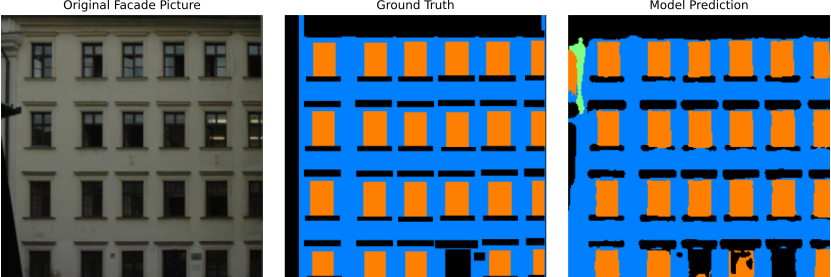
\includegraphics[width=\linewidth]{demo.pdf}
  \caption{Example (from \texttt{demo.ipynb}) showing the model prediction compared to ground truth on a held-out sample. For the final submission requirement, replace the input with a self-taken SKKU building photo and save it as \texttt{skku.jpg}, and export the predicted label image using the same palette format.}
  \label{fig:qualitative}
\end{figure}

\paragraph{Commentary}
Qualitatively, the model produces coherent and visually consistent segmentation results on the SKKU building image. Large facade regions are correctly identified, and repetitive structures such as windows are clearly and regularly segmented. This indicates that the network has learned meaningful architectural patterns and can effectively combine local texture information with global structural cues, aided by the U-Net skip connections and the transformer bottleneck that enlarges the receptive field.

The model works well mainly because the input image resembles the training distribution: a frontal viewpoint, clear facade geometry, and regularly arranged windows. Potential failure cases may occur in regions with occlusions (very clear for the trees in this sample), strong perspective distortion, or architectural styles not seen during training, where the learned geometric and texture features no longer match the visual statistics of the scene.